A new pirate sailing ship is being built. The ship has $N$ masts (poles) divided into unit sized segments~--- the height of a mast is equal to the number of its segments. Each mast is fitted with a number of sails and each sail exactly fits into one segment. Sails on one mast can be arbitrarily distributed among different segments, but each
segment can be fitted with at most one sail.

Different configurations of sails generate different amounts of thrust when exposed to the wind. Sails in front of other sails at the same height get less wind and contribute less thrust. For each sail we define its inefficiency as the total number of sails that are behind this sail and at the same height. Note that ``in front of'' and ``behind''
relate to the orientation of the ship: in the figure below, ``in front of'' means to the left, and ``behind'' means to the right.

The total inefficiency of a configuration is the sum of the inefficiencies of all individual sails.

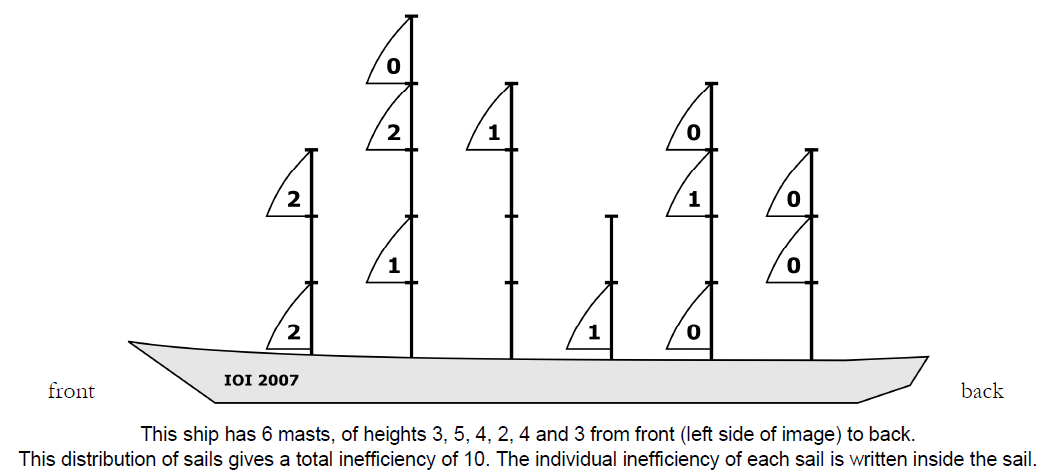
\includegraphics[scale=0.6]{sails.png}


Write a program that, given the height and the number of sails on each of the $N$ masts, determines the smallest possible total inefficiency.